% Analytical framework (fig:framework in the article). Compile with pdflatex.
\documentclass[border=4pt]{standalone}
\usepackage{tikz}
\usetikzlibrary{positioning,arrows.meta,calc}
\begin{document}
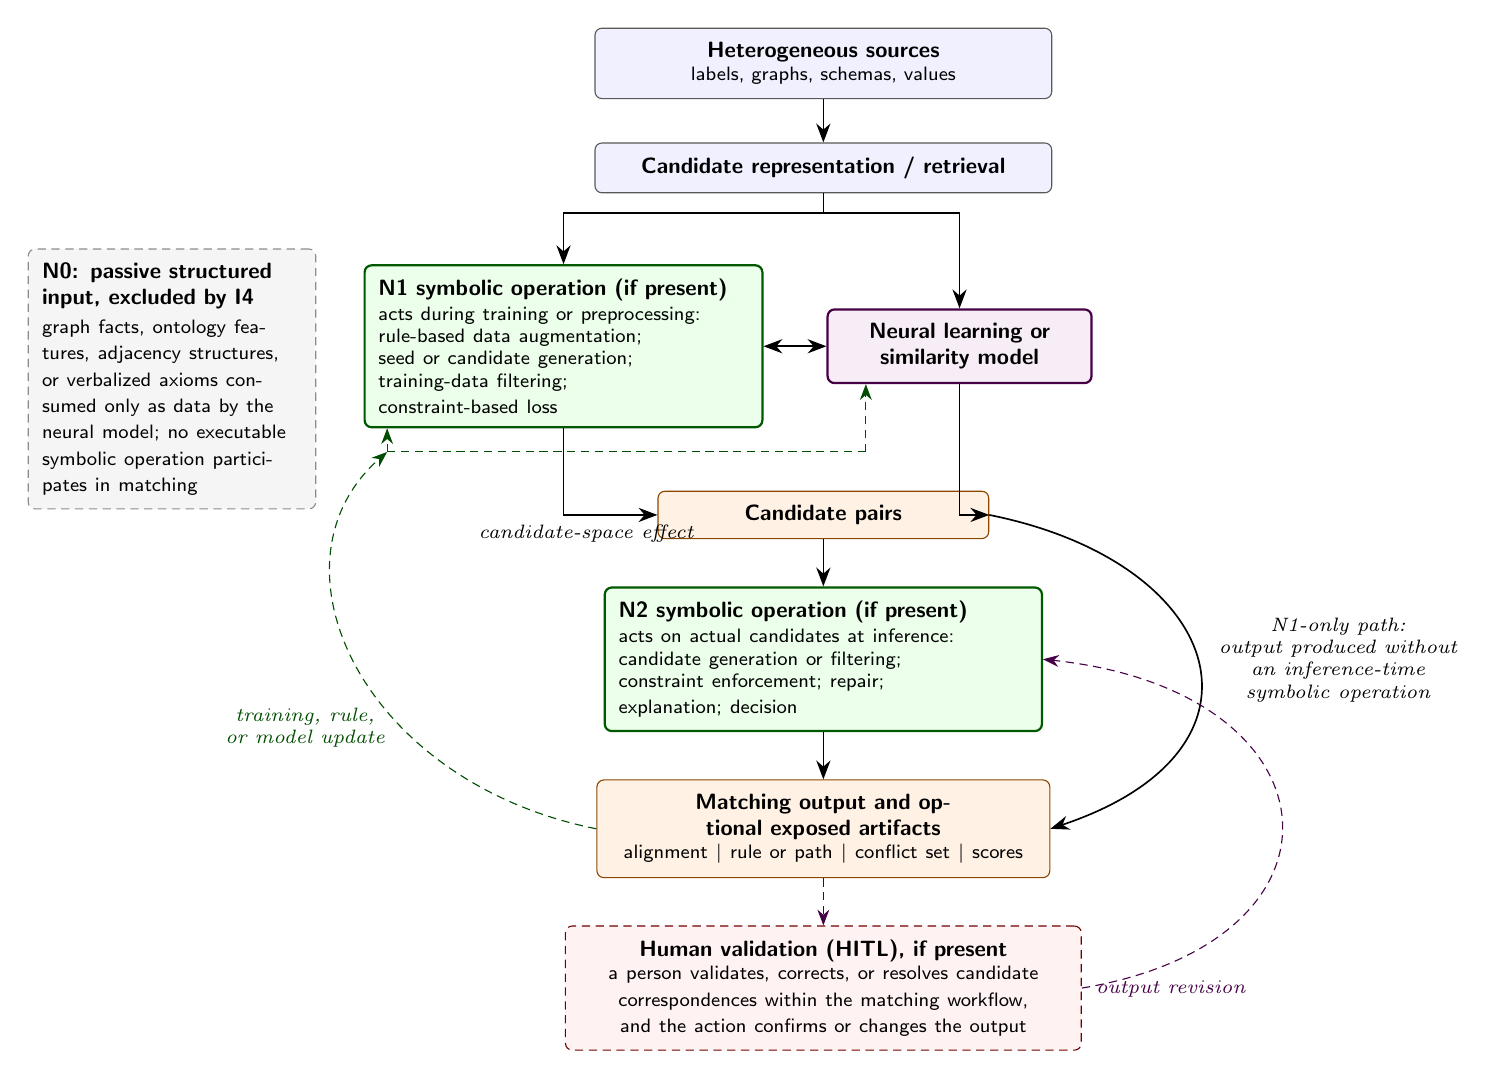
\begin{tikzpicture}[
  font=\footnotesize\sffamily,
  box/.style={draw, rounded corners=2.5pt, align=center, inner sep=5pt},
  proc/.style={box, fill=blue!6, draw=black!65, minimum width=58mm},
  symb/.style={box, fill=green!8, draw=green!35!black, thick},
  neur/.style={box, fill=violet!7, draw=violet!55!black, thick},
  arti/.style={box, fill=orange!10, draw=orange!55!black},
  hitl/.style={box, fill=red!5, draw=red!45!black, densely dashed},
  note/.style={box, fill=black!4, draw=black!45, densely dashed, align=left},
  flow/.style={-{Stealth[length=2.4mm]}, semithick},
  fb/.style={-{Stealth[length=2mm]}, densely dashed, green!30!black},
  rev/.style={-{Stealth[length=2mm]}, densely dashed, violet!55!black},
  lab/.style={font=\scriptsize\itshape, align=center},
]

\node[proc] (src) {\textbf{Heterogeneous sources}\\[-1pt]
  {\scriptsize labels, graphs, schemas, values}};
\node[proc, below=5.5mm of src] (repr)
  {\textbf{Candidate representation / retrieval}};

\node[symb, below=9mm of repr, xshift=-33mm, text width=47mm, align=left] (n1)
  {\textbf{N1 symbolic operation (if present)}\\[1pt]
  {\scriptsize acts during training or preprocessing:\\
  rule-based data augmentation;\\
  seed or candidate generation;\\
  training-data filtering;\\
  constraint-based loss}};
\node[neur, right=8mm of n1, text width=30mm] (nn)
  {\textbf{Neural learning or similarity model}};

\node[arti, minimum width=42mm] (pairs) at ($(repr.south |- n1.south)+(0,-11mm)$) {\textbf{Candidate pairs}};

\node[symb, below=6mm of pairs, text width=52mm, align=left] (n2)
  {\textbf{N2 symbolic operation (if present)}\\[1pt]
  {\scriptsize acts on actual candidates at inference:\\
  candidate generation or filtering;\\
  constraint enforcement; repair;\\
  explanation; decision}};

\node[arti, below=6mm of n2, text width=54mm] (dec)
  {\textbf{Matching output and optional exposed artifacts}\\[-1pt]
  {\scriptsize alignment $\mid$ rule or path $\mid$ conflict set $\mid$ scores}};

\node[hitl, below=6mm of dec, text width=62mm] (hv)
  {\textbf{Human validation (HITL), if present}\\[-1pt]
  {\scriptsize a person validates, corrects, or resolves candidate
  correspondences within the matching workflow, and the action
  confirms or changes the output}};

\node[note, text width=33mm, anchor=north east] (n0) at ($(n1.north west)+(-6mm,2mm)$)
  {\textbf{N0: passive structured input, excluded by I4}\\[1pt]
  {\scriptsize graph facts, ontology features, adjacency structures, or
  verbalized axioms consumed only as data by the neural model; no executable
  symbolic operation participates in matching}};

\draw[flow] (src) -- (repr);
\draw[flow] (repr.south) -- ++(0,-2.5mm) -| (n1.north);
\draw[flow] (repr.south) -- ++(0,-2.5mm) -| (nn.north);
\draw[flow, {Stealth[length=2.4mm]}-{Stealth[length=2.4mm]}] (n1.east) -- (nn.west);
\draw[flow] (n1.south) |- node[lab, pos=0.62, below] {candidate-space effect} (pairs.west);
\draw[flow] (nn.south) |- (pairs.east);
\draw[flow] (pairs) -- (n2);
\draw[flow] (n2) -- (dec);
\draw[rev] (dec) -- (hv);
\draw[flow] (pairs.east) .. controls +(30mm,-6mm) and +(30mm,10mm) ..
  node[lab, right, xshift=1.5mm] {N1-only path:\\ output produced without\\ an inference-time\\ symbolic operation} (dec.east);
\coordinate (bl) at ($(n1.south west)+(3mm,-3mm)$);
\coordinate (br) at ($(nn.west |- n1.south)+(5mm,-3mm)$);
\draw[fb] (dec.west) .. controls +(-30mm,6mm) and +(-16mm,-14mm) .. (bl)
  node[lab, pos=0.35, left, xshift=-1mm] {training, rule,\\ or model update};
\draw[fb, -] (bl) -- (br);
\draw[fb] (bl) -- ($(n1.south west)+(3mm,0)$);
\draw[fb] (br) -- ($(nn.south west)+(5mm,0)$);
\draw[rev] (hv.east) .. controls +(36mm,6mm) and +(38mm,-4mm) .. (n2.east)
  node[lab, pos=0.12, below, yshift=-1mm] {output revision};
\end{tikzpicture}
\end{document}
